\section{Design}

\textit{[I designkapitlet presenterar ni er implementation: skisser, lösningsförslag, hur lösningen utvecklats genom iterationer och motiverar era designbeslut med stöd från teori och resultat.]}

\textit{[Strukturera kapitlet så att det är tydligt hur designen utvecklats. Fokusera på de viktiga designbesluten och motivera dem. För mindre viktiga ändringar, hänvisa till bilagor.]}


\subsection{Designkoncept}

\textit{[Beskriv det övergripande designkonceptet]}

Det övergripande designkonceptet baseras på [beskriv huvudidé]. Gränssnittet riktar sig till [målgrupp] och ska främst stödja [huvudsakliga uppgifter].

Designen följer principerna om [t.ex. visibility, feedback, constraints från kurslitteraturen] för att säkerställa god användbarhet.


\subsection{Iteration 1: Tidiga skisser}

I den första iterationen skapades flera olika designalternativ. Figur \ref{fig:tidiga_skisser}, \ref{fig:tidiga3} och \ref{fig:tidiga_2} visar exempel på tidiga pappersprototyper.

\begin{figure}[H]
    \centering
    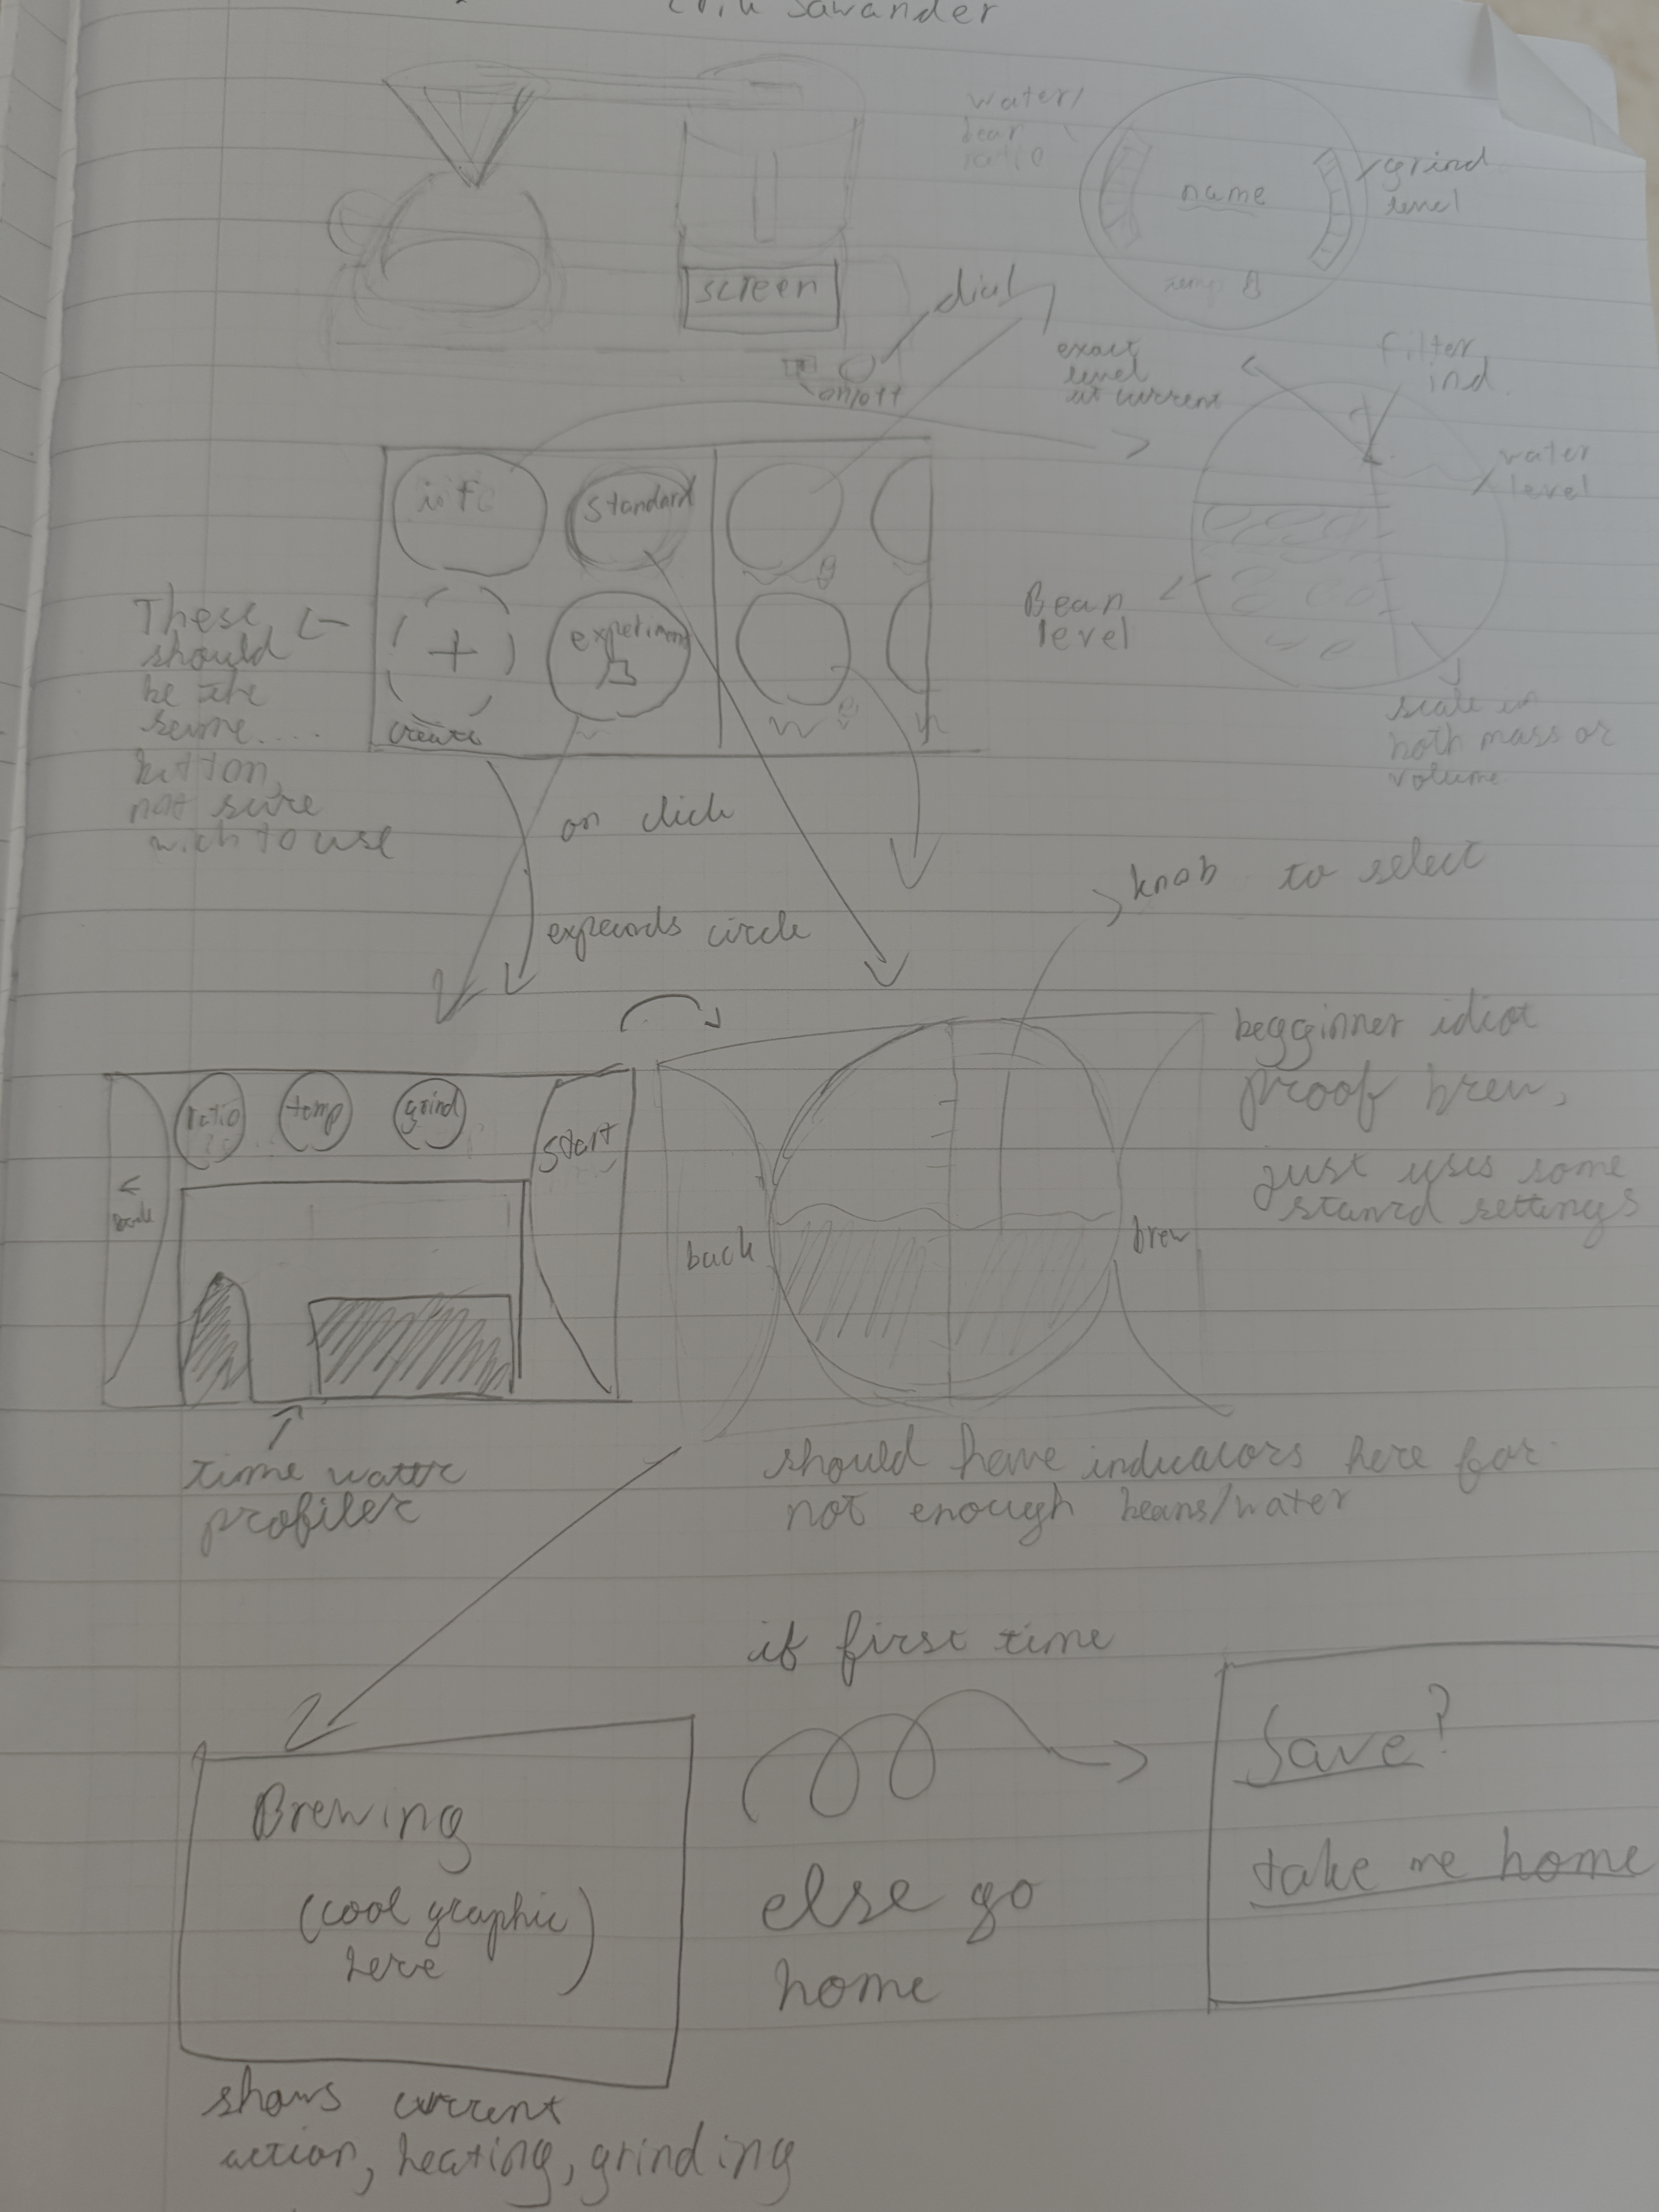
\includegraphics[width=0.8\textwidth]{bilder/paper.png}
    \caption{Tidig pappersprototyper från design studio-sessionen}
    \label{fig:tidiga_skisser}
\end{figure}

\begin{figure}[H]
    \centering
    \includegraphics[width=0.8\textwidth]{bilder/victor1.png}
    \includegraphics[width=0.8\textwidth]{bilder/victor2.png}
    \includegraphics[width=0.8\textwidth]{bilder/victor3.png}
    \caption{Tidig prototyp från design studio-sessionen}
    \label{fig:tidiga_2}
\end{figure}

\begin{figure}[H]
    \centering
    \includegraphics[width=0.8\textwidth]{bilder/sjov.png}
    \includegraphics[width=0.8\textwidth]{bilder/sjov2.png}
    \caption{Tidig prorotyp från design studio-sessionen}
    \label{fig:tidiga3}
\end{figure}

\textbf{Designalternativ A} fokuserade på ett touchscreen-baserat gränsnit med stora kreativa grafiska representationer för information. Syftet var att skapa något tydligt som ändå hanterade avancerade inställningar väl. Detta alternativ valdes bort eftersom representationerna hade dålig överensstämmelse med mentala modellen som en typisk användare har, och var istället mer anpassat till de som redan har kunskap inom avancerat kaffe bryggning.

Exempelvis så fokuserade gränsnitet på förhålanden mellan bönor och vatten, och i termer av massa. Redan inom gruppen skappade detta förvirring, då det inte va uppenbart hur mycket man ska brygga för att få en kopp, och om det skulla göra kaffet svagare eller inte.

Det beslutades dock att id\'eerna var rimliga för ett "advanced mode" i framtida iterationer.

\textbf{Designalternativ B} erbjöd ett alternativ som använde sig av fysiska knappar och reglage. All navigation styrdes av ett hjul. Att välja alternativ var mer intuitivt, men reglagen gjorde det svårare att använda avancerade inställningarna, och var inte praktiskt för att namnge profiler. 

\textbf{Designalternativ C} fokuserade på touch, och tillämpade en “plattare” design. Fler alternativ, inställningar, och funktioner kunde visas, och färre steg var obligatoriska för att brygga kaffe. Därför valdes det att basera första digitala prototypen på detta alternativ.
\subsection{Iteration 2: Första digitala prototyp}

\textit{[Beskriv utvecklingen till digital prototyp]}

Baserat på feedback från lo-fi-testerna utvecklades den första digitala prototypen. Huvudsakliga vyer inkluderar: startsidan, sidmenyn, “manage profiles”, “schedule coffee”, "create profile" och inställningar. 

\subsubsection{Startsida}

Startsidan designades för att [syfte]. Layouten följer [designprincip] genom att...

\begin{figure}[H]
    \centering
    \includegraphics[width=0.6\textwidth]{bilder/start.png}
    \caption{Första versionen av startsidan}
    \label{fig:startsida_v1}
\end{figure}

Huvudelementen är:
\begin{itemize}
    \item \textbf{Navigation}: Placerad i [position] för att...
    \item \textbf{Sökfunktion}: Synligt placerad eftersom användarnas huvuduppgift är...
    \item \textbf{Content area}: ...
\end{itemize}


\subsubsection{Manage Profiles}

Startsidan designades för att [syfte]. Layouten följer [designprincip] genom att...

\begin{figure}[H]
    \centering
    \includegraphics[width=0.6\textwidth]{bilder/manage.png}
    \caption{Första versionen av "manage profles" sidan}
    \label{fig:manage_v1}
\end{figure}

Huvudelementen är:
\begin{itemize}
    \item \textbf{Navigation}: Placerad i [position] för att...
    \item \textbf{Sökfunktion}: Synligt placerad eftersom användarnas huvuduppgift är...
    \item \textbf{Content area}: ...
\end{itemize}


\subsubsection{Schedule Coffee}

Startsidan designades för att [syfte]. Layouten följer [designprincip] genom att...

\begin{figure}[H]
    \centering
    \includegraphics[width=0.6\textwidth]{bilder/schedule.png}
    \caption{Första versionen av "schedule coffee" sidan}
    \label{fig:schedule_v1}
\end{figure}

Huvudelementen är:
\begin{itemize}
    \item \textbf{Navigation}: Placerad i [position] för att...
    \item \textbf{Sökfunktion}: Synligt placerad eftersom användarnas huvuduppgift är...
    \item \textbf{Content area}: ...
\end{itemize}
\subsubsection{Create Profile}

Startsidan designades för att [syfte]. Layouten följer [designprincip] genom att...

\begin{figure}[H]
    \centering
    \includegraphics[width=0.6\textwidth]{bilder/brew.png}
    \includegraphics[width=0.6\textwidth]{bilder/advancedshit.png}
    \caption{Första versionen av "create profiles" sidan}
    \label{fig:create_v1}
\end{figure}

Huvudelementen är:
\begin{itemize}
    \item \textbf{Navigation}: Placerad i [position] för att...
    \item \textbf{Sökfunktion}: Synligt placerad eftersom användarnas huvuduppgift är...
    \item \textbf{Content area}: ...
\end{itemize}
\subsubsection{ inställningar }

Startsidan designades för att [syfte]. Layouten följer [designprincip] genom att...

\begin{figure}[H]
    \centering
    \includegraphics[width=0.6\textwidth]{bilder/settings.png}
    \caption{Första versionen av inställningar }
    \label{fig:settings_v1}
\end{figure}

Huvudelementen är:
\begin{itemize}
    \item \textbf{Navigation}: Placerad i [position] för att...
    \item \textbf{Sökfunktion}: Synligt placerad eftersom användarnas huvuduppgift är...
    \item \textbf{Content area}: ...
\end{itemize}

\subsubsection{Sidmenyn}

Startsidan designades för att [syfte]. Layouten följer [designprincip] genom att...

Huvudelementen är:
\begin{itemize}
    \item \textbf{Navigation}: Placerad i [position] för att...
    \item \textbf{Sökfunktion}: Synligt placerad eftersom användarnas huvuduppgift är...
    \item \textbf{Content area}: ...
\end{itemize}
\subsection{Iteration 3: Förfinad design}

\textit{[Beskriv hur designen förbättrades baserat på utvärdering]}

Efter användbarhetstester i iteration 2 identifierades flera problem (se avsnitt \ref{sec:resultat_test}). Följande ändringar gjordes:

\textbf{Problem 1:} Användare hade svårt att hitta [funktion]

\textbf{Lösning:} [Funktion] flyttades till [position] och fick en mer framträdande visuell design (se figur \ref{fig:forbattring1}).

\begin{figure}[h]
    \centering
    % \includegraphics[width=\textwidth]{bilder/before_after.png}
    \caption{Före (vänster) och efter (höger) designändring}
    \label{fig:forbattring1}
\end{figure}

\textbf{Motivering:} Ändringen baseras på designprincipen om visibility \cite{sharp2019} och testresultaten visade att [beskriv förbättring].


\subsection{Slutgiltig design}

\textit{[Presentera den slutgiltiga designen]}

Den slutgiltiga designen är resultat av [antal] iterationer och integrerar feedback från [antal] användare. Fullständiga vyer finns i Bilaga C.

Huvudsakliga designprinciper som tillämpats:
\begin{itemize}
    \item \textbf{Konsistens}: Alla vyer följer samma layoutmönster...
    \item \textbf{Feedback}: Användaren får tydlig återkoppling när...
    \item \textbf{Affordance}: Interaktiva element signalerar tydligt...
\end{itemize}


\subsection{Designbeslut och motiveringar}

\textit{[Sammanfatta viktiga designbeslut]}

\begin{table}[h]
\centering
\begin{tabular}{|p{4cm}|p{5cm}|p{4cm}|}
\hline
\textbf{Designbeslut} & \textbf{Motivering} & \textbf{Teoretisk grund} \\
\hline
Navigation i top bar & Användarna förväntar sig... & Mental modeller \cite{sharp2019} \\
\hline
Färgschema: ... & Tillgänglighet och kontrast & WCAG-riktlinjer \\
\hline
... & ... & ... \\
\hline
\end{tabular}
\caption{Sammanställning av huvudsakliga designbeslut}
\end{table}
